\documentclass[tikz,border=10pt]{standalone}
\begin{document}
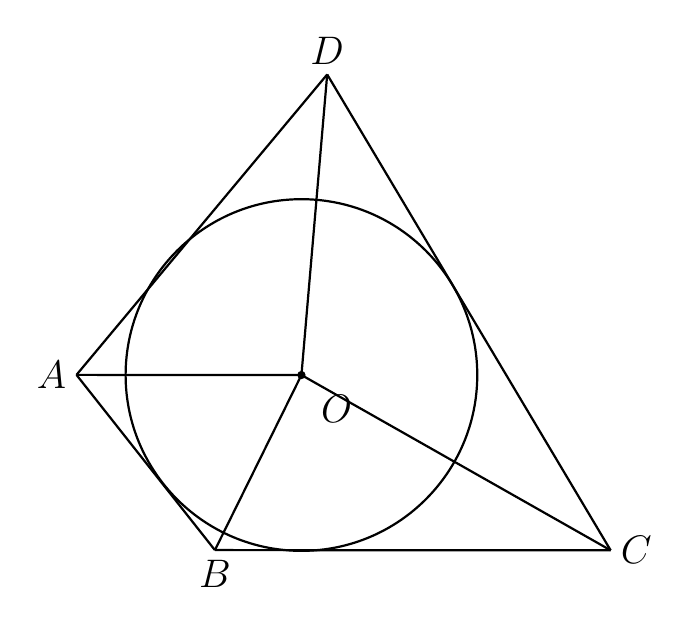
\begin{tikzpicture}[line join=round, line width=0.8pt]
% Named coordinates: s = 0.013491 cm/px, centre = ink bbox centre (320.5, 289.5), y flipped
\coordinate (D) at (-0.22799999999999998,3.026);
\coordinate (A) at (-3.412002526136905,-0.7893352162403799);
\coordinate (O) at (-0.555,-0.791);
\coordinate (C) at (3.3719985640211534,-3.0174643316409764);
\coordinate (B) at (-1.6539985640211534,-3.0145356683590245);

% Incircle centred at O, radius 165.56 px = 2.233 cm
\draw (O) circle (2.233cm);

% Solid segments
\draw (D) -- (C);   % DC
\draw (B) -- (C);   % BC
\draw (A) -- (D);   % AD
\draw (D) -- (O);   % DO
\draw (A) -- (O);   % AO
\draw (O) -- (C);   % OC
\draw (A) -- (B);   % AB
\draw (O) -- (B);   % OB

% Centre dot at O
\fill (O) circle (1.5pt);

% Labels (cap height 28 px -> 15.5 pt font)
\node[above, font=\fontsize{15.5}{18.6}\selectfont] at (D) {$D$};
\node[left,  font=\fontsize{15.5}{18.6}\selectfont] at (A) {$A$};
% O label: manual offset below-right of the dot, clear of line OC
\node[anchor=north west, xshift=0.12cm, yshift=-0.12cm, font=\fontsize{15.5}{18.6}\selectfont] at (O) {$O$};
\node[right, font=\fontsize{15.5}{18.6}\selectfont] at (C) {$C$};
\node[below, font=\fontsize{15.5}{18.6}\selectfont] at (B) {$B$};
\end{tikzpicture}
\end{document}
% GEOAGENT_REPAIR_V1 fb95c09946135974 2c6b58e51b560a5e1af5951ae9847eabe673d27df8ec29bd732b134498e9140f
